\documentclass[12pt]{article}
\usepackage[utf8]{inputenc}
\usepackage[utf8]{inputenc}
\usepackage{amsmath}
\usepackage{amsthm}
\usepackage{amssymb}
\usepackage{geometry}
\usepackage{amsfonts}
\usepackage{mathrsfs}
\usepackage{bm}
\usepackage{hyperref}
\usepackage[dvipsnames]{xcolor}
\usepackage[inline]{enumitem}
\usepackage{mathtools}
\usepackage{changepage}
\usepackage{graphicx}
\usepackage{caption}
\usepackage{subcaption}
\usepackage{lipsum}
\usepackage{tikz}
\usetikzlibrary{matrix, patterns, decorations.pathreplacing, calligraphy}
\usepackage{tikz-cd}
\usepackage[nameinlink]{cleveref}
\geometry{
headheight=15pt,
left=60pt,
right=60pt
}
\setlength{\emergencystretch}{20pt}
\usepackage{fancyhdr}
\pagestyle{fancy}
\fancyhf{}
\lhead{}
\chead{Section 4.5 Exercises}
\rhead{\thepage}
\hypersetup{
    colorlinks=true,
    linkcolor=blue,
    urlcolor=blue
}

\theoremstyle{definition}
\newtheorem*{remark}{Remark}

\newtheoremstyle{exercise}
    {}
    {}
    {}
    {}
    {\bfseries}
    {.}
    { }
    {\thmname{#1}\thmnumber{#2}\thmnote{ (#3)}}
\theoremstyle{exercise}
\newtheorem{exercise}{Exercise 4.5.}

\newtheoremstyle{solution}
    {}
    {}
    {}
    {}
    {\itshape\color{magenta}}
    {.}
    { }
    {\thmname{#1}\thmnote{ #3}}
\theoremstyle{solution}
\newtheorem*{solution}{Solution}

\Crefformat{exercise}{#2Exercise 4.5.#1#3}

\newcommand{\interior}[1]{%
  {\kern0pt#1}^{\mathrm{o}}%
}
\newcommand{\ts}{\textsuperscript}
\newcommand{\setcomp}[1]{#1^{\mathsf{c}}}
\newcommand{\quand}{\quad \text{and} \quad}
\newcommand{\N}{\mathbf{N}}
\newcommand{\Z}{\mathbf{Z}}
\newcommand{\Q}{\mathbf{Q}}
\newcommand{\I}{\mathbf{I}}
\newcommand{\R}{\mathbf{R}}
\newcommand{\C}{\mathbf{C}}

\DeclarePairedDelimiter\abs{\lvert}{\rvert}
% Swap the definition of \abs* and \norm*, so that \abs
% and \norm resizes the size of the brackets, and the 
% starred version does not.
\makeatletter
\let\oldabs\abs
\def\abs{\@ifstar{\oldabs}{\oldabs*}}
%
\let\oldnorm\norm
\def\norm{\@ifstar{\oldnorm}{\oldnorm*}}
\makeatother

\DeclarePairedDelimiter\paren{(}{)}
\makeatletter
\let\oldparen\paren
\def\paren{\@ifstar{\oldparen}{\oldparen*}}
\makeatother

\DeclarePairedDelimiter\bkt{[}{]}
\makeatletter
\let\oldbkt\bkt
\def\bkt{\@ifstar{\oldbkt}{\oldbkt*}}
\makeatother

\DeclarePairedDelimiter\set{\{}{\}}
\makeatletter
\let\oldset\set
\def\set{\@ifstar{\oldset}{\oldset*}}
\makeatother

\setlist[enumerate,1]{label={(\alph*)}}

\begin{document}

\section{Section 4.5 Exercises}

Exercises with solutions from Section 4.5 of \hyperlink{ua}{[UA]}.

\begin{exercise}
\label{ex:1}
    Show how the Intermediate Value Theorem follows as a corollary to Theorem 4.5.2.
\end{exercise}

\begin{solution}
    Let \( f : [a, b] \to \R \) be continuous and let \( L \in \R \) be such that either \( f(a) < L < f(b) \) or \( f(b) < L < f(a) \); our aim is to show that there exists \( c \in (a, b) \) such that \( f(c) = L \). Theorem 3.4.7 shows that \( [a, b] \) is connected and hence Theorem 4.5.2 implies that the image \( f([a, b]) \) is also connected. Clearly \( f(a), f(b) \in f([a, b]) \), so Theorem 3.4.7 implies that \( L \in f([a, b]) \), i.e.\ there exists \( c \in [a, b] \) such that \( f(c) = L \). In fact, since \( f(a) \neq L \) and \( f(b) \neq L \) we have \( c \in (a, b) \).
\end{solution}

\begin{exercise}
\label{ex:2}
    Provide an example of each of the following, or explain why the request is impossible
    \begin{enumerate}
        \item A continuous function defined on an open interval with range equal to a closed interval.

        \item A continuous function defined on a closed interval with range equal to an open interval.

        \item A continuous function defined on an open interval with range equal to an unbounded closed set different from \( \R \).

        \item A continuous function defined on all of \( \R \) with range equal to \( \Q \).
    \end{enumerate}
\end{exercise}

\begin{solution}
    (I am not sure if Abbott allows unbounded intervals here!)
    \begin{enumerate}
        \item If we allow unbounded intervals, then \( f : \R \to \R \) given by \( f(x) = x \) is an example of such a function. For bounded intervals, see \href{https://lew98.github.io/Mathematics/UA_Section_4_4_Exercises.pdf}{Exercise 4.4.8 (b)} for an example of such a function.
        
        \item If we allow unbounded intervals, then \( f : \R \to \R \) given by \( f(x) = x \) is an example of such a function. If we do not allow unbounded intervals, then such a function cannot exist by Theorem 4.4.1 (Preservation of Compact Sets).

        \item If we allow unbounded intervals, then \( f : \R \to \R \) given by \( f(x) = \max \{ 0, x \} \) is an example of such a function; the image of \( f \) is \( [0, \infty) \). For bounded intervals, consider the function \( f : (0, 2) \to \R \) given by \( f(x) = \tfrac{1}{x(2 - x)} \); the image of \( f \) is \( [1, \infty) \).

        \item This is impossible. \( \R \) is connected (Theorem 3.4.7) and so its image under a continuous function must also be connected (Theorem 4.5.2); however, \( \Q \) is not connected (Theorem 3.4.7).
    \end{enumerate}
\end{solution}

\begin{exercise}
\label{ex:3}
    A function \( f \) is \textit{increasing} on \( A \) if \( f(x) \leq f(y) \) for all \( x < y \) in \( A \). Show that if \( f \) is increasing on \( [a, b] \) and satisfies the intermediate value property (Definition 4.5.3), then \( f \) is continuous on \( [a, b] \).
\end{exercise}

\begin{solution}
    First, let us prove the following lemma.
    
    \vspace{2mm}

    \noindent \textbf{Lemma 1.} Suppose \( a < b \) and \( f : [a, b] \to \R \) is increasing.
    \begin{enumerate}[label = (\roman*)]
        \item If \( c \in (a, b] \), then
        \[
            \lim_{x \to c^-} f(x) = \sup \{ f(x) : a < x < c \}.
        \]

        \item If \( c \in [a, b) \), then
        \[
            \lim_{x \to c^+} f(x) = \inf \{ f(x) : c < x < b \}.
        \]
    \end{enumerate}

    \noindent \textit{Proof.}
    \begin{enumerate}[label = (\roman*)]
        \item Fix \( c \in (a, b] \). Note that since \( f \) is increasing, we have \( f([a, b]) \subseteq [f(a), f(b)] \); it follows that \( \{ f(x) : a < x < c \} \) is bounded and non-empty, so \( S := \sup \{ f(x) : a < x < c \} \) exists. Let \( \epsilon > 0 \) be given. There exists a \( y \in (a, c) \) such that \( S - \epsilon < f(y) \leq S \). Since \( f \) is increasing, we then have
        \[
            x \in (y, c) \implies S - \epsilon < f(y) \leq f(x) \leq S.
        \]
        In other words, letting \( \delta = c - y \), for any \( x \) satisfying \( c - \delta < x < c \) we have \( \abs{f(x) - S} < \epsilon \). It follows that \( \lim_{x \to c^-} f(x) = S \).

        \item The proof is similar to part (i). \qed
    \end{enumerate}

    Returning to the exercise, we will now prove the contrapositive result: if \( f \) is increasing and not continuous on \( [a, b] \), then \( f \) does not satisfy the intermediate value property. Suppose therefore that \( f \) is not continuous at some \( c \in [a, b] \) i.e.\ suppose that \( \lim_{x \to c} f(x) \neq f(c) \) (Theorem 4.3.2 (iv)).
    \begin{description}
        \item[Case 1.] Suppose \( c \in (a, b) \). Since \( f \) is increasing on \( [a, b] \), Lemma 1 implies that both of the one-sided limits exist:
        \begin{gather*}
            \alpha := \lim_{x \to c^-} f(x) = \sup \{ f(x) : a < x < c \}, \\[2mm]
            \beta := \lim_{x \to c^+} f(x) = \inf \{ f(x) : c < x < b \}.
        \end{gather*}
        By \href{https://lew98.github.io/Mathematics/UA_Section_4_2_Exercises.pdf}{Exercise 4.2.10 (b)}, it must be the case that at least one of these limits is not equal to \( f(c) \). Since \( f \) is increasing, we must then have \( \alpha < \beta \); it follows that the infinite subset \( (\alpha, \beta) \setminus \{ f(c) \} \subsetneq [f(a), f(b)] \) does not belong to the image of \( f \) and so \( f \) does not satisfy the intermediate value property on \( [a, b] \).

        \item[Case 2.] Suppose \( c = a \), i.e.\ \( f \) is not continuous at \( a \). Since \( f \) is increasing on \( [a, b] \), Lemma 1 implies that the limit from the right exists:
        \[
            \beta := \lim_{x \to a^+} f(x) = \inf \{ f(x) : a < x < b \}.
        \]
        Since \( a \) is the minimum element of the domain of \( f \), we have \( \lim_{x \to a} f(x) = \lim_{x \to a^+} f(x) = \beta \), and since \( f \) is not continuous at \( a \) and increasing on \( [a, b] \), it must then be the case that \( f(a) < \beta \). It follows that the infinite subset \( (f(a), \beta) \subsetneq [f(a), f(b)] \) does not belong to the image of \( f \) and so \( f \) does not satisfy the intermediate value property on \( [a, b] \).

        \item[Case 3.] If \( f \) fails to be continuous at \( b \), then an argument similar to the one given in Case 2, this time using the limit from the left, shows that \( f \) does not satisfy the intermediate value property on \( [a, b] \).
    \end{description}
\end{solution}

\begin{exercise}
\label{ex:4}
    Let \( g \) be continuous on an interval \( A \) and let \( F \) be the set of points where \( g \) fails to be one-to-one; that is,
    \[
        F = \{ x \in A : f(x) = f(y) \text{ for some } y \neq x \text{ and } y \in A \}.
    \]
    Show \( F \) is either empty or uncountable.
\end{exercise}

\begin{solution}
    It will suffice to show that if \( F \) is not empty then \( F \) is uncountable. Suppose therefore that there exist \( x < y \) in \( A \) such that \( g(x) = g(y) \). If \( g \) is constant on \( [x, y] \), then \( F \) contains the uncountable subset \( [x, y] \) and so must itself be uncountable. Otherwise, there exists some \( a \in (x, y) \) such that \( g(a) \neq g(x) \). Let
    \[
        I := \left( \min \{ g(x), g(a) \}, \max \{ g(x), g(a) \} \right)
    \]
    and note that \( I \) is a proper interval (not a singleton) since \( g(a) \neq g(x) \). Since \( g \) is continuous on \( A \), the Intermediate Value Theorem (Theorem 4.5.1) implies that for each \( t \in I \) there exist \( x_t \in (x, a) \) and \( y_t \in (a, y) \) such that \( g(x_t) = g(y_t) = t \), so that \( x_t \in F \). Since \( g \) is a function, each \( t \in I \) gives rise to a distinct \( x_t \in F \); since \( I \) is uncountable, it then follows that \( F \) is uncountable.
\end{solution}

\begin{exercise}
\label{ex:5}
    \begin{enumerate}
        \item Finish the proof of the Intermediate Value Theorem using the Axiom of Completeness started previously.

        \item Finish the proof of the Intermediate Value Theorem using the Nested Interval Property started previously.
    \end{enumerate}
\end{exercise}

\begin{solution}
    \begin{enumerate}
        \item (Here is the start of the proof from the textbook.) To simplify matters a bit, let's consider the special case where \( f \) is a continuous function satisfying \( f(a) < 0 < f(b) \) and show that \( f(c) = 0 \) for some \( c \in (a, b) \). First let
        \[
            K = \{ x \in [a, b] : f(x) \leq 0 \}.
        \]
        Notice that \( K \) is bounded above by \( b \), and \( a \in K \) so \( K \) is not empty. Thus we may appeal to the Axiom of Completeness to assert that \( c = \sup K \) exists.

        There are three cases to consider:
        \[
            f(c) > 0, \,\, f(c) < 0, \text{  and  } f(c) = 0.
        \]
        \begin{description}
            \item[Case 1.] Suppose that \( f(c) > 0 \). Then since \( f \) is continuous at \( c \), there is a \( \delta > 0 \) such that \( f(x) > 0 \) for all \( x \in (c - \delta, c + \delta) \cap [a, b] \) (see \href{https://lew98.github.io/Mathematics/UA_Section_4_3_Exercises.pdf}{Exercise 4.3.8 (c)}). This implies the existence of a \( t \in (c - \delta, c) \cap [a, b] \) such that \( t \) is an upper bound of \( K \), which contradicts that \( c \) is the supremum of \( K \).

            \item[Case 2.] Suppose that \( f(c) < 0 \). Then since \( f \) is continuous at \( c \), there is a \( \delta > 0 \) such that \( f(x) < 0 \) for all \( x \in (c - \delta, c + \delta) \cap [a, b] \) (see \href{https://lew98.github.io/Mathematics/UA_Section_4_3_Exercises.pdf}{Exercise 4.3.8 (c)}). This implies the existence of a \( t \in (c, c + \delta) \cap [a, b] \) such that \( t \) belongs to \( K \), which contradicts that \( c \) is the supremum of \( K \).
        \end{description}
        So the only possibility is that \( f(c) = 0 \); note that \( c \) lies strictly between \( a \) and \( b \) since \( f(a) < 0 < f(b) \).

        The more general statement of the Intermediate Value Theorem can be obtained from this special case by considering either the function \( g(x) = f(x) - L \) if \( f(a) < f(b) \) or the function \( g(x) = L - f(x) \) if \( f(a) > f(b) \).

        \item (Here is the start of the proof from the textbook.) Again, consider the special case where \( L = 0 \) and \( f(a) < 0 < f(b) \). Let \( I_0 = [a, b] \), and consider the midpoint
        \[
            z = (a + b)/2.
        \]
        If \( f(z) \geq 0 \), then set \( a_1 = a \) and \( b_1 = z \). If \( f(z) < 0 \), then set \( a_1 = z \) and \( b_1 = b \). In either case, the interval \( I_1 = [a_1, b_1] \) has the property that \( f \) is negative at the left endpoint and nonnegative at the right. 

        We repeat this procedure inductively, obtaining a sequence \( (I_n = [a_n, b_n]) \) of nested intervals such that \( f(a_n) < 0, f(b_n) \geq 0 \), and \( \abs{I_n} = 2^{-n}(b - a) \) for all \( n \in \N \). We can now appeal to the Nested Interval Property to assert that \( \bigcap_{n=1}^{\infty} I_n = \{ c \} \) for some \( c \in [a, b] \) (the intersection is non-empty as the intervals are closed and nested, and the intersection is a singleton since \( \lim \abs{I_n} = 0 \)); furthermore, we have \( \lim a_n = \lim b_n = c \). Since \( f \) is continuous at \( c \), it follows that \( \lim f(a_n) = \lim f(b_n) = f(c) \). The Order Limit Theorem implies that \( f(c) \leq 0 \), since \( f(a_n) < 0 \) for all \( n \in \N \), and that \( f(c) \geq 0 \), since \( f(b_n) \geq 0 \) for all \( n \in \N \). Thus \( f(c) = 0 \). 
        
        Again, \( c \) lies strictly between \( a \) and \( b \) since \( f(a) < 0 < f(b) \), and the more general statement of the Intermediate Value Theorem can be obtained from this special case by considering either the function \( g(x) = f(x) - L \) if \( f(a) < f(b) \) or the function \( g(x) = L - f(x) \) if \( f(a) > f(b) \).
    \end{enumerate}
\end{solution}

\begin{exercise}
\label{ex:6}
    Let \( f : [0, 1] \to \R \) be continuous with \( f(0) = f(1) \).
    \begin{enumerate}
        \item Show that there must exist \( x, y \in [0, 1] \) satisfying \( \abs{x - y} = 1/2 \) and \( f(x) = f(y) \).

        \item Show that for each \( n \in \N \) there exist \( x_n, y_n \in [0, 1] \) with \( \abs{x_n - y_n} = 1/n \) and \( f(x_n) = f(y_n) \).

        \item If \( h \in (0, 1/2) \) is not of the form \( 1/n \), there does not necessarily exist \( \abs{x - y} = h \) satisfying \( f(x) = f(y) \). Provide an example that illustrates this using \( h = 2/5 \).
    \end{enumerate}
\end{exercise}

\begin{solution}
    \begin{enumerate}
        \item Define \( g : \bkt{0, \tfrac{1}{2}} \to \R \) by \( g(x) = f(x) - f \paren{x + \tfrac{1}{2}} \) and note that \( g \) is continuous by Theorems 4.3.4 and 4.3.9. If \( g(0) = 0 \) then \( f(0) = f \paren{\tfrac{1}{2}} \) and we are done. Otherwise, note that
        \[
            g(0) = f(0) - f \paren{\tfrac{1}{2}} = f(1) - f \paren{\tfrac{1}{2}} = -\paren{f \paren{\tfrac{1}{2}} - f(1)} = -g \paren{\tfrac{1}{2}}.
        \]
        Thus \( 0 \in \paren{\min \set{ g(0), g \paren{\tfrac{1}{2}}}, \max \set{ g(0), g \paren{\tfrac{1}{2}} }} \) and so the Intermediate Value Theorem implies that there exists a \( c \in \paren{ 0, \tfrac{1}{2} } \) such that \( g(c) = 0 \), i.e.\ \( f(c) = f \paren{ c + \tfrac{1}{2} } \).

        \item For \( n = 1 \), we can take \( x_1 = 0 \) and \( y_1 = 1 \). For \( n \geq 2 \), define \( g : \bkt{0, \tfrac{n-1}{n}} \to \R \) by \( g(x) = f(x) - f \paren{x + \tfrac{1}{n}} \) and note that \( g \) is continuous by Theorems 4.3.4 and 4.3.9. If \( g(0) = 0 \) then \( f(0) = f \paren{\tfrac{1}{n}} \) and we are done. Otherwise, note that
        \begin{align*}
            g(0) &= f(0) - f \paren{\tfrac{1}{n}}, \\
            g \paren{\tfrac{1}{n}} &= f \paren{\tfrac{1}{n}} - f \paren{\tfrac{2}{n}}, \\
            g \paren{\tfrac{2}{n}} &= f \paren{\tfrac{2}{n}} - f \paren{\tfrac{3}{n}}, \\
            \vdots & \\
            g \paren{\tfrac{n-1}{n}} &= f \paren{\tfrac{n-1}{n}} - f(1).
        \end{align*}
        Since \( f(0) = f(1) \), this implies that
        \[
            g(0) + g \paren{\tfrac{1}{n}} + g \paren{\tfrac{2}{n}} + \cdots + g \paren{\tfrac{n-1}{n}} = 0,
        \]
        and since \( g(0) \neq 0 \), there must exist some \( k \in \{ 1, \ldots, n - 1 \} \) such that \( g \paren{\tfrac{k}{n}} \) has the opposite sign to \( g(0) \). The Intermediate Value Theorem now implies that there exists a \( c \in \paren{0, \tfrac{k}{n}} \) such that \( g(c) = 0 \), i.e.\ \( f(c) = f \paren{c + \tfrac{1}{n}} \). Thus we can take \( x_n = c \) and \( y_n = c + \tfrac{1}{n} \).

        \item Consider the function \( f : [0, 1] \to \R \) given by
        \[
            f(x) = \begin{cases}
                -10 x & \text{if } 0 \leq x < \tfrac{1}{5}, \\
                15 \paren{x - \tfrac{1}{5}} - 2 & \text{if } \tfrac{1}{5} \leq x < \tfrac{2}{5}, \\
                -10 \paren{x - \tfrac{2}{5}} + 1 & \text{if } \tfrac{2}{5} \leq x < \tfrac{3}{5}, \\
                15 \paren{x - \tfrac{3}{5}} - 1 & \text{if } \tfrac{3}{5} \leq x < \tfrac{4}{5}, \\
                -10 \paren{x - \tfrac{4}{5}} + 2 & \text{if } \tfrac{4}{5} \leq x \leq 1. \\
            \end{cases}
        \]
        This function has the property that \( f \paren{x + \tfrac{2}{5}} - f(x) = 1 \) for every \( x \in \bkt{0, \tfrac{3}{5}} \) (see \Cref{fig:1}), so that there cannot possibly exist \( x, y \in [0, 1] \) satisfying \( \abs{x - y} = \tfrac{2}{5} \) and \( f(x) = f(y) \).

        \begin{figure}[ht]
            \centering
            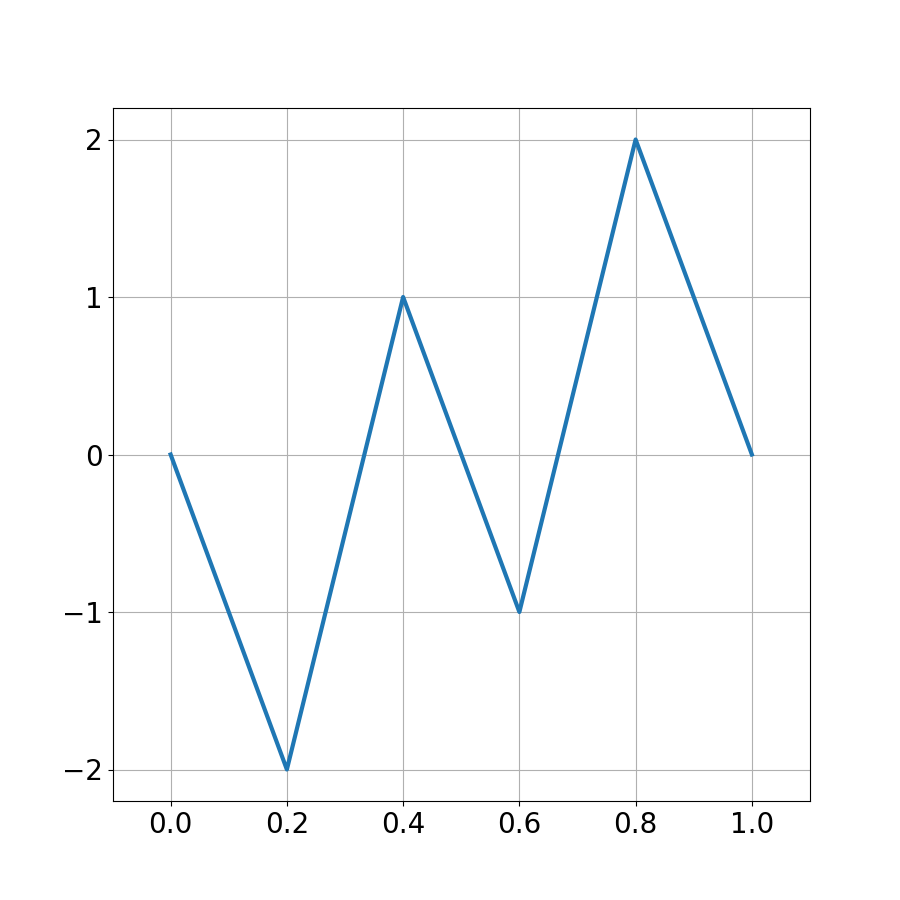
\includegraphics[width=14cm]{UA_Section_4_5_Figure_1.png}
            \caption{\Cref{ex:6} (c) function}
            \label{fig:1}
        \end{figure}
    \end{enumerate}
\end{solution}

\begin{exercise}
\label{ex:7}
    Let \( f \) be a continuous function on the closed interval \( [0, 1] \) with range also contained in \( [0, 1] \). Prove that \( f \) must have a fixed point; that is, show \( f(x) = x \) for at least one value of \( x \in [0, 1] \).
\end{exercise}

\begin{solution}
    Define \( g : [0, 1] \to \R \) by \( g(x) = f(x) - x \) and note that \( g \) is continuous by Theorem 4.3.4. Furthermore, fixed points of \( f \) correspond precisely to zeros of \( g \). If \( g(0) = 0 \) or \( g(1) = 0 \), then we are done. Suppose therefore that \( g(0) \neq 0 \) and \( g(1) \neq 0 \). Since \( 0 \leq f(x) \leq 1 \) for all \( x \in [0, 1] \), it must then be the case that \( 0 < f(0) \leq 1 \) and \( 0 \leq f(1) < 1 \), which implies that \( g(0) \) is positive and \( g(1) \) is negative. The Intermediate Value Theorem can now be applied to obtain some \( x \in (0, 1) \) such that \( g(x) = 0 \).
\end{solution}

\begin{exercise}[Inverse functions]
\label{ex:8}
    If a function \( f : A \to \R \) is one-to-one, then we can define the inverse function \( f^{-1} \) on the range of \( f \) in the natural way: \( f^{-1}(y) = x \) where \( y = f(x) \).

    Show that if \( f \) is continuous on an interval \( [a, b] \) and one-to-one, then \( f^{-1} \) is also continuous.
\end{exercise}

\begin{solution}
    Here are a couple of useful lemmas.

    \vspace{2mm}

    \noindent \textbf{Lemma 2.} Suppose \( f : A \to \R \) is continuous and injective, where \( A \subseteq \R \) is some domain. Then \( f \) is strictly monotone, i.e.\ \( f \) is either strictly increasing or strictly decreasing.

    \vspace{2mm}

    \noindent \textit{Proof.} We will prove the contrapositive result: if \( f \) is continuous and neither strictly increasing nor strictly decreasing, then \( f \) is not injective.

    Since \( f \) is not strictly increasing, there exist \( x < y \) in \( A \) such that \( f(y) \leq f(x) \), and since \( f \) is not strictly decreasing, there exist \( s < t \) in \( A \) such that \( f(s) \leq f(t) \). There are a number of cases to check. We will check one case only; the others are handled similarly.

    Suppose that \( x < s < t \) and \( f(s) < f(x) < f(t) \). Since \( f \) is continuous, the Intermediate Value Theorem implies the existence of some \( c \in (s, t) \), so that \( c \neq x \), such that \( f(c) = f(x) \). Thus \( f \) is not injective. \qed

    \vspace{2mm}

    \noindent \textbf{Lemma 3.} Suppose \( g : A \to I \) is a strictly monotone surjection, where \( A \subseteq \R \) is some domain and \( I \) is an interval. Then \( g \) is continuous.

    \vspace{2mm}

    \noindent \textit{Proof.} The cases where \( I \) is empty or a singleton (which are precisely the cases where \( A \) is empty or a singleton, respectively) are easily handled, so we may assume that \( I \) is a proper interval. We may also assume that \( g \) is strictly increasing (if \( g \) is strictly decreasing, consider the function \( -g \) instead).

    Fix \( b \in A \) and \( \epsilon > 0 \). We consider four cases.
    \begin{description}
        \item[Case 1.] Suppose \( g(b) - \epsilon \) and \( g(b) + \epsilon \) both belong to \( I \). Since \( g \) is a surjection, there exist \( a, c \in A \) such that \( g(a) = g(b) - \epsilon \) and \( g(c) = g(b) + \epsilon \), and since \( g \) is strictly increasing it must be the case that \( a < b < c \). Set \( \delta = \min \{ b - a, c - b \} \). Then
        \[
            x \in (b - \delta, b + \delta) \cap A \implies g(x) \in (g(b) - \epsilon, g(b) + \epsilon)
        \]
        also follows since \( g \) is strictly increasing.

        \item[Case 2.] Suppose \( g(b) - \epsilon \in I \) and \( g(b) + \epsilon \not\in I \). Since \( g \) is a surjection, there is an \( a \in A \) such that \( g(a) = g(b) - \epsilon \), and since \( I \) is an interval it must be the case that \( I \) is bounded above by \( g(b) + \epsilon \), so that \( \sup I \) exists and is less than or equal to \( g(b) + \epsilon \).

        If \( g(b) = \sup I \), then let \( \delta = b - a \) and note that \( \delta \) is positive since \( g(a) = g(b) - \epsilon < g(b) \) implies \( a < b \) by the monotonicity of \( g \). Since \( g(b) \) is the supremum of the image of \( g \) and \( g \) is strictly increasing, we then have
        \[
            x \in (b - \delta, b + \delta) \cap A \implies g(x) \in (g(b) - \epsilon, g(b)] \subseteq (g(b) - \epsilon, g(b) + \epsilon).
        \]
        
        If \( g(b) < \sup I \), then since \( I \) is an interval we have \( s := \tfrac{g(b) + \sup I}{2} \in I \). The surjectivity of \( g \) then implies that there exists a \( c \in A \) such that \( g(c) = s \). Since \( g \) is strictly increasing and \( g(b) - \epsilon < g(b) < s \), we must have \( a < b < c \). Set \( \delta = \min \{ b - a, c - b \} \). Then
        \[
            x \in (b - \delta, b + \delta) \cap A \implies g(x) \in (g(b) - \epsilon, g(b) + \epsilon)
        \]
        also follows since \( g \) is strictly increasing.

        \item[Case 3.] The case where \( g(b) - \epsilon \not\in I \) and \( g(b) + \epsilon \in I \) is handled similarly to Case 2, this time by considering the infimum of \( I \).

        \item[Case 4.] The case where neither one of \( g(b) - \epsilon \) and \( g(b) + \epsilon \) belongs to \( I \) is handled similarly to Cases 2 and 3, by considering both the infimum and supremum of \( I \). Note that since \( I \) is a proper interval, we must have \( \inf I < \sup I \), so that \( g(b) \) could never be equal to both \( \inf I \) and \( \sup I \).
    \end{description}

    In any case, we obtain a \( \delta > 0 \) such that
    \[
        x \in (b - \delta, b + \delta) \cap A \implies g(x) \in (g(b) - \epsilon, g(b) + \epsilon),
    \]
    so that \( g \) is continuous at each \( b \in A \). \qed

    \vspace{2mm}

    Returning to the exercise, we have a continuous and bijective function \( f : [a, b] \to f([a, b]) \) defined on the compact and connected set \( [a, b] \) (we may as well assume \( a < b \)); the image of \( f \) must be compact and connected (Theorems 4.4.1 and 4.5.2). The only possibility is \( f([a, b]) = [c, d] \) for some \( c < d \) (Theorems 3.3.8 and 3.4.7). It must be the case that \( c \) is strictly less than \( d \) since \( f \) is injective.

    Now let \( g : [c, d] \to [a, b] \) be the inverse of \( f \). By Lemma 2, \( f \) must be strictly monotone; it is straightforward to verify that the inverse of a strictly monotone function is also strictly monotone. Since the image of \( g \) is the interval \( [a, b] \), we may apply Lemma 3 to conclude that \( g \) is continuous.
\end{solution}

\noindent \hrulefill

\noindent \hypertarget{ua}{\textcolor{blue}{[UA]} Abbott, S. (2015) \textit{Understanding Analysis.} 2\ts{nd} edition.}

\end{document}